\begin{figure}[tbp]
  \centering
  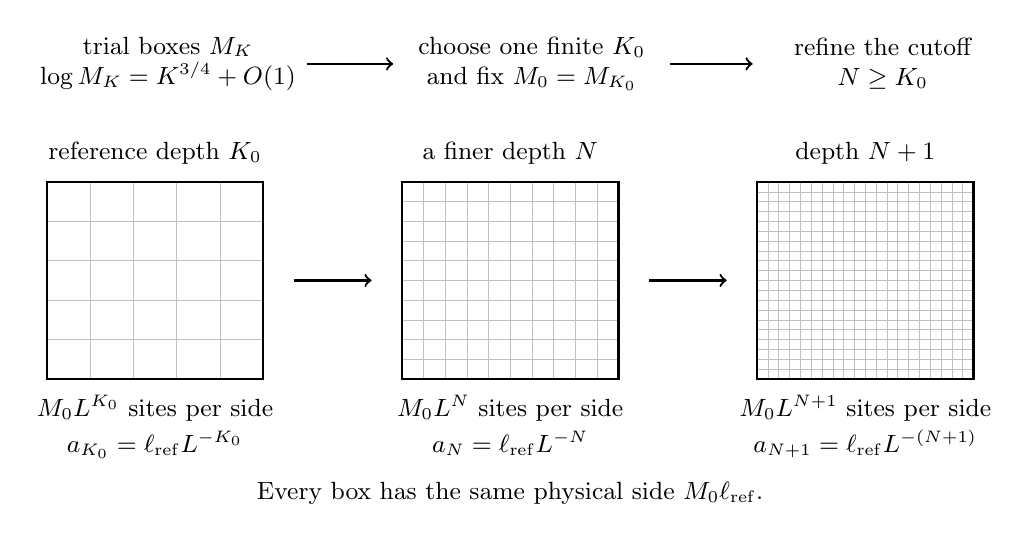
\begin{tikzpicture}[x=1.1cm,y=1cm,font=\small]
    \node[align=center] at (1.4,4.0)
      {trial boxes $M_K$\\$\log M_K=K^{3/4}+O(1)$};
    \draw[->,thick] (3.0,4.0) -- (4.0,4.0);
    \node[align=center] at (5.6,4.0)
      {choose one finite $K_0$\\and fix $M_0=M_{K_0}$};
    \draw[->,thick] (7.2,4.0) -- (8.15,4.0);
    \node[align=center] at (9.65,4.0)
      {refine the cutoff\\$N\ge K_0$};

    \begin{scope}[shift={(0,0)}]
      \draw[step=0.5,black!25,very thin] (0,0) grid (2.5,2.5);
      \draw[thick] (0,0) rectangle (2.5,2.5);
      \node[above] at (1.25,2.6) {reference depth $K_0$};
      \node[align=center,below] at (1.25,-0.08)
        {$M_0L^{K_0}$ sites per side\\[2pt]$a_{K_0}=\ell_{\mathrm{ref}}L^{-K_0}$};
    \end{scope}
    \draw[->,thick] (2.85,1.25) -- (3.75,1.25);
    \begin{scope}[shift={(4.1,0)}]
      \draw[step=0.25,black!25,very thin] (0,0) grid (2.5,2.5);
      \draw[thick] (0,0) rectangle (2.5,2.5);
      \node[above] at (1.25,2.6) {a finer depth $N$};
      \node[align=center,below] at (1.25,-0.08)
        {$M_0L^N$ sites per side\\[2pt]$a_N=\ell_{\mathrm{ref}}L^{-N}$};
    \end{scope}
    \draw[->,thick] (6.95,1.25) -- (7.85,1.25);
    \begin{scope}[shift={(8.2,0)}]
      \draw[step=0.125,black!25,very thin] (0,0) grid (2.5,2.5);
      \draw[thick] (0,0) rectangle (2.5,2.5);
      \node[above] at (1.25,2.6) {depth $N+1$};
      \node[align=center,below] at (1.25,-0.08)
        {$M_0L^{N+1}$ sites per side\\[2pt]$a_{N+1}=\ell_{\mathrm{ref}}L^{-(N+1)}$};
    \end{scope}
    \node at (5.35,-1.45)
      {Every box has the same physical side $M_0\ell_{\mathrm{ref}}$.};
  \end{tikzpicture}\par\medskip
  \caption{The order of choices in the lower-bound argument.
  The growing family of trial boxes is used only to select one
  reference depth and one coarse period. The comparison then transfers
  the small square-box test to all finer admitted cutoffs at the same
  terminal coupling. The grids are schematic; their counts are not
  the actual lattice periods. Refinement does not enlarge the physical
  reference box.}
  \label{fig:fixed-reference-box}
\end{figure}
